\documentclass[aspectratio=169,11pt]{beamer}
\usepackage{presentation-theme}
\title{Pair-to-single information flow with pair distogram supervision}
\author{Wuhao}
\hypersetup{pdftitle={Pair-to-single information flow with pair distogram supervision},
  pdfauthor={Wuhao},pdfsubject={MassSpecGym pilot, waves 1--6, 1 October 2026}}
\definecolor{teal}{HTML}{087F8C}
\definecolor{ochre}{HTML}{A86B17}
\newcommand{\bodytext}[4]{\node[anchor=north west,inner sep=0,align=left,text width=#3cm,font=\figurefont\fontsize{9.2}{11.5}\selectfont] at (#1,#2) {#4};}
\newcommand{\plotfigure}[1]{\node[anchor=north,inner sep=0] at (8,6.85) {\includegraphics[width=14.5cm,height=4.6cm,keepaspectratio]{figures/#1.pdf}};}
\newcommand{\tableat}[3]{\node[anchor=north west,inner sep=0,font=\figurefont\fontsize{#2}{10.5}\selectfont] at (.9,#1) {#3};}
\begin{document}

\begin{frame}
\begin{tikzpicture}[remember picture,overlay,shift={(current page.south west)}]
\header{RESEARCH WORKLOG / 1 OCT 2026 / WAVES 1--6}{Supervise pairs, then move their content into singles}
\bodytext{.9}{6.65}{13.8}{\textbf{Current candidate:} pair distogram supervision with attention bias, mean pair values and edge-gated messages. Arm: \texttt{dual\_bias\_mean\_gated}.}
\foreach \x/\value/\label in {2.7/{0.731}/{Single MACCS AUC},8/{0.748}/{Pair MACCS AUC},13.1/{26.8\%}/{Single retrieval top-1}}{
  \node[font=\brandmedium\fontsize{30}{34}\selectfont,text=teal] at (\x,4.65) {\value};
  \node[font=\figurefont\fontsize{10}{12}\selectfont] at (\x,3.85) {\label};
}
\bodytext{.9}{3.02}{13.8}{At $C=256$, the candidate improves the reported comparisons with independent models and the old joint recipe at both 2 and 0.1 Da. The final comparison uses seed 0 only.}
\takeaway{The next check is multi-seed confirmation of the matched-width candidate.}
\source{Source throughout: docs/pair\_single\_dual\_20261001.md. Headline: wave 6, D256/C256, 0.1 Da, 20k steps, seed 0, test fold. Results are pilot measurements.}
\end{tikzpicture}
\end{frame}

\begin{frame}
\begin{tikzpicture}[remember picture,overlay,shift={(current page.south west)}]
\header{01 / DIAGNOSIS}{Attention bias can route values without carrying pair content}
\eqn[14]{1.0}{6.6}{a_{ij}=\operatorname{softmax}_j\!\left(\frac{q_i^\top k_j}{\sqrt d}+b(z_{ij})\right),\qquad u_i=\sum_j a_{ij}v_j}
\eqn[14]{1.0}{5.15}{\frac{\partial u_i}{\partial b_{ij}}=a_{ij}(v_j-u_i)}
\bodytext{1}{3.7}{6.5}{\textbf{Content bottleneck}\\The value is always a single-stream vector. Similar neighbour values suppress the pair effect.}
\bodytext{8.2}{3.7}{6.7}{\textbf{Training bottleneck}\\The old joint objective reads only singles. Its distogram is built from single predictor latents.}
\takeaway{A useful pair state needs both a direct learning signal and a channel into singles.}
\source{Worklog §§2--3. Derivative holds singles fixed. Pair features are compressed to one routing scalar per attention head; saturated softmax further weakens gradients.}
\end{tikzpicture}
\end{frame}

\begin{frame}
\begin{tikzpicture}[remember picture,overlay,shift={(current page.south west)}]
\header{02 / OBJECTIVE}{One context encoder, two supervised predictor branches}
\diagramblock{2.25}{5.65}{2.5}{1.05}{Context encoder\\$\operatorname{Enc}_{\theta}$}
\diagramblock{6.6}{6.25}{2.25}{.85}{Singles $s^{(L)}$}
\diagramblock{6.6}{4.25}{2.25}{.85}{Pairs $z^{(L)}$}
\diagramblock{11.35}{6.25}{3.9}{.85}{Single predictor $P_s$\\Masked $m/z$ cross-entropy}
\diagramblock{11.35}{4.25}{3.9}{.85}{Pair predictor $P_z$\\Pair-distogram cross-entropy}
\draw[arr] (3.6,5.9)--(5.35,6.25);
\draw[arr] (3.6,5.4)--(5.35,4.25);
\draw[arr] (7.85,6.25)--(9.25,6.25);
\draw[arr] (7.85,4.25)--(9.25,4.25);
\draw[arr,draw=teal] (6.6,4.78)--(6.6,5.7);
\node[anchor=west,text=teal,font=\figurefont\fontsize{8}{10}\selectfont] at (6.85,5.25) {bridge in each encoder block};
\eqn[13]{1.05}{2.9}{\mathcal L_{\mathrm{dual}}=0.7\mathcal L_{\mathrm{MAE}}(P_s(s^{(L)}))+0.3\mathcal L_{\mathrm{dist}}(P_z(z^{(L)}))}
\takeaway{Keep the 0.7 / 0.3 loss weights; put the distogram gradient on the pair branch.}
\source{Worklog §§3--4. Black arrows: forward computation. Teal: pair-to-single content within encoder blocks (schematic). Both branches update the shared encoder.}
\end{tikzpicture}
\end{frame}

\begin{frame}
\begin{tikzpicture}[remember picture,overlay,shift={(current page.south west)}]
\header{03 / INTERFACES}{Bias, mean values and gated messages have different roles}
\bodytext{1}{6.6}{3.85}{\textbf{Attention bias}\\Changes neighbour weights. Helps the single-stream retrieval geometry.}
\bodytext{5.85}{6.6}{4.0}{\textbf{Mean pair values}\\Adds pooled pair content directly to the single residual stream.}
\bodytext{10.7}{6.6}{4.25}{\textbf{Edge-gated messages}\\Pairs gate channels of neighbour messages, plus a direct pair-value term.}
\eqn[11]{1}{4.6}{m_i=\frac1n\sum_j\sigma(G\bar z_{ij}+g)\odot V\operatorname{RMSNorm}(s_j)+P\frac1n\sum_j\bar z_{ij}}
\eqn[12]{1}{3.65}{\Delta s_i=\gamma\odot\operatorname{RMSNorm}(W_o m_i)}
\bodytext{1}{2.85}{13.8}{IPA-style values reuse attention routing to pool pairs. The final candidate combines bias, a mean-first value bridge and the gated bridge above.}
\takeaway{Use bias for routing and direct bridges to transport pair content.}
\source{Worklog §5 and wave 2. $\bar z=\operatorname{RMSNorm}(z)$; $n$ valid tokens; bridge rank 64; learned channel scale initialised to 0.1. Roles are interpretations of ablations.}
\end{tikzpicture}
\end{frame}

\begin{frame}
\begin{tikzpicture}[remember picture,overlay,shift={(current page.south west)}]
\header{04 / PROTOCOL}{Compare prediction, chemistry and retrieval separately}
\bodytext{1}{6.6}{6.55}{\textbf{Training}\\MassSpecGym 1.5; 31 sorted peaks + CLS.\\194,119 train / 19,429 val / 17,556 test spectra; molecule-disjoint folds.\\[7pt]Base: D256/C128, six blocks, four heads.\\20k steps, batch 128, AdamW, bf16.\\Same examples, masks and joint initialisation.}
\bodytext{8.3}{6.6}{6.5}{\textbf{Evaluation}\\Masked $m/z$ CE and pair-distogram CE.\\MACCS ridge probes: 8,192 train spectra; penalty selection on 4,096 val spectra.\\[7pt]Test fold + 1,494 unused validation molecules (confirm).\\Cosine retrieval on train-standardised features.}
\bodytext{1}{2.7}{13.8}{\textbf{Evidence levels:} wave 1 has three seeds. New interfaces, capacity controls, masking, bin sizes and matched-width conclusions are seed-0 follow-ups.}
\takeaway{Compare cross-entropy only within a fixed bin width; keep test and confirm results distinct.}
\source{Worklog §§6, 8--10. Random masking: 60\% context, 25\% targets (at most 8). Single readout = peak mean + CLS; pair readout pools peak--peak and both CLS directions.}
\end{tikzpicture}
\end{frame}

\begin{frame}
\begin{tikzpicture}[remember picture,overlay,shift={(current page.south west)}]
\header{05 / WAVE 1 / THREE SEEDS}{Direct pair values improve the single readout}
\plotfigure{wave1}
\takeaway{IPA gives the best retrieval and masked prediction; mean values give the best test chemistry.}
\source{Worklog §8, per-arm means: D256/C128, 2 Da, 20k steps, three seeds. Points are means, without error bars; paired seed ranges follow. Single-only pair readout is a random-feature control.}
\end{tikzpicture}
\end{frame}

\begin{frame}
\begin{tikzpicture}[remember picture,overlay,shift={(current page.south west)}]
\header{06 / PAIRED EVIDENCE}{The gains repeat across seeds; bridge content is used}
\bodytext{1}{6.55}{13.8}{\textbf{IPA minus old joint: mean [minimum, maximum] over three matched seeds}}
\tableat{5.85}{10}{\begin{tabular}{@{}lrr@{}}\toprule
Metric & Test / validation & Confirm \\\midrule
Masked $m/z$ CE & $-0.018\;[-0.021,-0.016]$ & --- \\
Single MACCS AUC & $+0.021\;[+0.018,+0.022]$ & $+0.018\;[+0.011,+0.026]$ \\
Single retrieval top-1 & $+3.6\;[+2.7,+4.1]$ pp & $+5.7\;[+5.1,+6.4]$ pp \\\bottomrule
\end{tabular}}
\bodytext{1}{3.35}{6.5}{\textbf{Bridge intervention}\\Mask-matched shuffling raises MAE CE by 0.056--0.062. Zeroing raises it by about 0.051.}
\bodytext{8.25}{3.35}{6.6}{\textbf{Remaining trade-off}\\IPA pair-distogram CE is 0.012 worse than pair-only; confirm pair AUC has a seed range that crosses zero.}
\takeaway{Three seeds support the single-stream gains; they do not establish every pair-side improvement.}
\source{Worklog §8, paired differences and interventions. Ranges are seed minima/maxima, not confidence intervals. Prediction uses fixed validation masks. Pair-only confirm AUC delta: +0.003 [−0.001,+0.008].}
\end{tikzpicture}
\end{frame}

\begin{frame}
\begin{tikzpicture}[remember picture,overlay,shift={(current page.south west)}]
\header{07 / CAPACITY CONTROL / SEED 0}{Wider pairs change the baseline comparison}
\plotfigure{capacity}
\takeaway{Use C256 on both pair branches before claiming an advantage over pair-only.}
\source{Worklog §8, pair-only capacity controls. C256/L6: 11.4M parameters, 21.5 steps/s; C128 dual: about 12M, about 13 steps/s in the cited comparison. Width matching does not match total parameters.}
\end{tikzpicture}
\end{frame}

\begin{frame}
\begin{tikzpicture}[remember picture,overlay,shift={(current page.south west)}]
\header{08 / WAVE 5 / C256 / 2 Da / SEED 0}{The combined bridge clears the matched-width baselines}
\tableat{6.65}{9.3}{\begin{tabular}{@{}lrrrrrr@{}}\toprule
Arm & MAE $\downarrow$ & Dist $\downarrow$ & sAUC t/c $\uparrow$ & pAUC t/c $\uparrow$ & s@1 t/c (\%) $\uparrow$ & Params \\\midrule
Single only & 2.614 & --- & .651/.645 & --- & 22.1/32.8 & 11.1M \\
Pair only & --- & 2.225 & --- & .712/.703 & --- & 11.4M \\
Old joint & 2.540 & --- & .664/.656 & .696/.684 & 24.7/35.4 & 18.5M \\
Dual / bias & 2.522 & 2.223 & .669/.658 & .719/.706 & 25.7/37.0 & 21.3M \\
Dual / bias + IPA & 2.503 & 2.222 & .686/.672 & .718/.700 & 25.5/37.9 & 21.5M \\
Dual / gated & 2.508 & 2.223 & .700/.692 & .716/.703 & 24.4/37.9 & 21.7M \\
\textcolor{teal}{Dual / bias + mean + gated} & 2.509 & 2.216 & .697/.682 & .726/.707 & 26.7/38.6 & 21.9M \\\bottomrule
\end{tabular}}
\bodytext{1}{2.9}{6.45}{\textbf{Versus single only}\\MAE $-0.105$; single AUC $+0.046$ test; top-1 $+4.6$ pp test.}
\bodytext{8.25}{2.9}{6.6}{\textbf{Versus pair only}\\Distogram $-0.009$; pair AUC $+0.014$ test and about $+0.003$ confirm.}
\takeaway{The broad win is promising; the confirm pair-AUC and distogram margins are small.}
\source{Worklog §8, wave 5. D256/C256, six blocks, 20k steps, seed 0; single-only uses D256. t/c = test/confirm; s/p = single/pair. Reported deltas may differ from rounded table subtraction.}
\end{tikzpicture}
\end{frame}

\begin{frame}
\begin{tikzpicture}[remember picture,overlay,shift={(current page.south west)}]
\header{09 / MASKING / SEED 0}{Span + isotope masking reduces chemistry-probe accuracy}
\plotfigure{masking}
\takeaway{Keep random masking for this recipe; retrieval gains do not offset the chemistry loss.}
\source{Worklog §9. Thompson intensity-weighted spans + isotope closure: visible target isotope partner 63.5\% → 0\%; mean target intensity 0.139 → 0.308. Test deltas, seed 0; pair-only has no single readout.}
\end{tikzpicture}
\end{frame}

\begin{frame}
\begin{tikzpicture}[remember picture,overlay,shift={(current page.south west)}]
\header{10 / BIN WIDTH / C128 / SEED 0}{Finer mass bins improve chemistry across model families}
\plotfigure{bins}
\takeaway{Use downstream probes to compare bin widths: 500, 5,000 and 10,000 classes have different CE scales.}
\source{Worklog §10. D256/C128, 20k steps, seed 0. Selected reported rows; the dual-mean series starts at 0.2 Da. Finer bins also enlarge prediction heads, so this is not a parameter-controlled comparison.}
\end{tikzpicture}
\end{frame}

\begin{frame}
\begin{tikzpicture}[remember picture,overlay,shift={(current page.south west)}]
\header{11 / WAVE 6 / C256 / 0.1 Da / SEED 0}{The candidate keeps the broad win at finer resolution}
\tableat{6.65}{9.3}{\begin{tabular}{@{}lrrrrrr@{}}\toprule
Arm & MAE $\downarrow$ & Dist $\downarrow$ & sAUC t/c $\uparrow$ & pAUC t/c $\uparrow$ & s@1 t/c (\%) $\uparrow$ & Params \\\midrule
Single only & 4.295 & --- & .691/.681 & --- & 23.7/35.5 & 16.0M \\
Pair only & --- & 3.3645 & --- & .737/.721 & --- & 13.8M \\
Old joint & 4.212 & --- & .723/.707 & .727/.710 & 26.6/38.0 & 23.4M \\
Dual / bias & 4.150 & 3.3596 & .721/.705 & .752/.732 & 26.5/39.1 & 26.2M \\
Dual / bias + mean & 4.139 & 3.3553 & .735/.718 & .752/.734 & 25.9/38.7 & 26.4M \\
Dual / bias + IPA & 4.125 & 3.3642 & .732/.720 & .750/.730 & 26.1/38.6 & 26.4M \\
Dual / gated & 4.152 & 3.3635 & .735/.721 & .752/.736 & 26.2/39.7 & 26.5M \\
\textcolor{teal}{Dual / bias + mean + gated} & 4.157 & 3.3569 & .731/.719 & .748/.732 & 26.8/40.2 & 26.7M \\\bottomrule
\end{tabular}}
\bodytext{1}{2.45}{13.8}{Versus old joint: lower MAE; higher single/pair AUC and retrieval on both folds.}
\takeaway{The combined bridge wins across baseline comparisons, although other dual arms lead individual metrics.}
\source{Worklog §10, wave 6. D256/C256, six blocks, 20k steps, seed 0. Combined bridge vs pair-only: distogram −0.0076; pair AUC +0.011/+0.011. Total model sizes differ.}
\end{tikzpicture}
\end{frame}

\begin{frame}
\begin{tikzpicture}[remember picture,overlay,shift={(current page.south west)}]
\header{12 / OTHER FOLLOW-UPS}{Longer training helps readouts; scale alone does not}
\bodytext{1}{6.55}{6.4}{\textbf{40k steps: readouts keep improving}\\IPA single test AUC 0.694; top-1 30.3\%.\\Pair-distogram CE 2.235 vs pair-only 2.234.\\MAE is 0.007 worse than old joint.\\[8pt]Prediction fit and downstream utility do not move together.}
\bodytext{8.25}{6.55}{6.55}{\textbf{D384/C192, eight blocks, 20k}\\Bridges still beat old joint.\\Bigger models do not beat base models on the reported downstream results.\\[8pt]More data or training may be needed; that explanation remains untested.}
\bodytext{1}{2.9}{13.8}{\textbf{Interface ablation:} removing bias improves chemistry but costs about 5 pp retrieval in the C128 comparison. Retaining the old single-latent distogram (dualplus) adds no clear benefit.}
\takeaway{Choose the interface for the joint chemistry-and-retrieval goal, then confirm it at the intended scale.}
\source{Worklog §8, wave 2: longer-training, scale and new-interface tables. All seed 0. 40k IPA vs old joint: +0.021 single AUC, +2.9 pp test top-1.}
\end{tikzpicture}
\end{frame}

\begin{frame}
\begin{tikzpicture}[remember picture,overlay,shift={(current page.south west)}]
\header{13 / DECISION AND NEXT EXPERIMENT}{Confirm the candidate before promoting the recipe}
\bodytext{1}{6.6}{13.8}{\textbf{Carry forward}\\D256/C256; dual 0.7 MAE + 0.3 pair distogram; bias + mean + gated; random masks; 0.1 Da bins. Keep single readouts for retrieval.}
\bodytext{1}{4.95}{13.8}{\textbf{Repeat the final comparison across seeds}\\Candidate, old joint, single only and pair only; matched examples, masks and training budget. Report paired changes in MAE, distogram, both AUCs and retrieval.}
\bodytext{1}{3.15}{13.8}{\textbf{Resolve the narrow margins}\\Prioritise pair-distogram and confirm pair-AUC differences. Track parameters and throughput; pair-width matching does not equal compute matching.}
\takeaway{Recommended candidate: dual\_bias\_mean\_gated. Final matched-width evidence: seed 0, pending replication.}
\source{Worklog §§8, 10--11. README includes the candidate command and source links; source document retains the original wave-1 reproduction example. No new training was run for this presentation.}
\end{tikzpicture}
\end{frame}

\end{document}
